% !TEX root = main.tex
\section{Constructing ranking functions}
\label{sec:ranking}

Although rankability implies almost-sure termination, the converse does not hold in general. For example,
\begin{equation}
\tif{{-}\tsample < 0}{\underline{0}}{(\tY \lambda x. x) \, \underline 0}
\label{ex:0 probability reachable}
\end{equation}
terminates in 3 steps with probability 1, but isn't rankable because $(\tY \lambda x. x) \, \underline 0$ is reachable, although that has probability 0. 
Not only is this counterexample AST, it's PAST. %positively almost surely terminating i.e.~the expected time to termination is finite.

A ranking function can be constructed under the stronger assumptions that, for every $N$ reachable from $M$, the expected number of $\tY$-reduction steps from $N$ to a value is finite. In particular, the expected number of $\tY$-reduction steps from each reachable term is a ranking function. Note that a finite number of expected $\tY$-reduction steps does not necessarily imply a finite number of expected total reduction steps.

\begin{example}
\label{ex:tY finite does not imply t finite}
The term
\[
M = \big(\tY \lambda f n. \tif{\tsample - 0.5 < 0}{n \, \underline 0}{f (\lambda x. n (n x))}\big) (\lambda x. x+1)
\] 
terminates with only 2 $\tY$-reductions on average i.e.~$\expect{T_M^\tY} = 2$, but applies the increment function $2^n$ times with probability $2^{-1-n}$ for $n \geq 0$, which diverges i.e.~$\expect{T_M} = \infty$.
\end{example}

\begin{theorem} \label{thm:minimal}
Given a closed term $M$, the function $f:Rch(M) \to \mathbb R$ given by 
\[
f(N) := \mathbb E [\text{number of }\tY\text{-reduction steps from }N\text{ to a value}]
\] 
if it exists, is the least of all possible ranking functions of $M$.
\end{theorem}
\begin{proof}
Let $f$ be the candidate least ranking function defined above, and suppose $g$ is another ranking function such that $f(N) > g(N)$ for some $N \in Rch(M)$. The restrictions of $f$ and $g$ to $Rch(N)$ have the same properties assumed of $f$ and $g$, so assume w.l.o.g.~that $N=M$. The difference $g - f$ is then a supermartingale (with the same setup as in the proof of %\Cref{thm:rankable gives supermartingale}
%Theorem \ref{rankable implies ast}) 
\Cref{thm:rankable and strict rankable});
therefore $\mathbb E[g(M_n)] \leq \mathbb E[f(M_n)] + g(M)-f(M)$, for all $n$.

We have $\mathbb E[f(M_n)] = \sum_{k=n}^\infty \mathbb P[M_k = E[\tY N] \text{ for some }E, N] \to 0 \text{ as } n \to \infty$; 
therefore as $g(M) - f(M) < 0$, eventually $\mathbb E[g(M_n)] < 0$, which is impossible. 
It follows that $g \geq f$ as required.

In order for $f$ to be the least ranking function of $M$, it also has to actually be a ranking function itself. Each of the conditions on a ranking function is easily verified from the definition of $f$.
\end{proof}

\subsection{Partial ranking functions}
Even in the case of reasonable simple terms, explicitly constructing a ranking function would be a lot of work, and \Cref{thm:minimal} makes even stronger assumptions than almost-sure termination, so it isn't useful for proving it.

\begin{example}[Geometric distribution]
Consider the term
\begin{align*}
&(\tY \lambda f, n. \\
&\quad \tif{\tsample - 0.5 < 0}{n}{f (n+1)} \\
&) \, \underline{0}
\end{align*}
which generates a geometric distribution (let $\Theta = \lambda f, n : \tif{\tsample \underline{- 0.5} < 0}{n}{f (n\underline{+ 1})}$, then the term is $(\tY \Theta)\ \underline 0$).
    Despite its simplicity, its $Rch$ contains all the terms: see \Cref{fig:geometric distribution}.
\begin{figure}
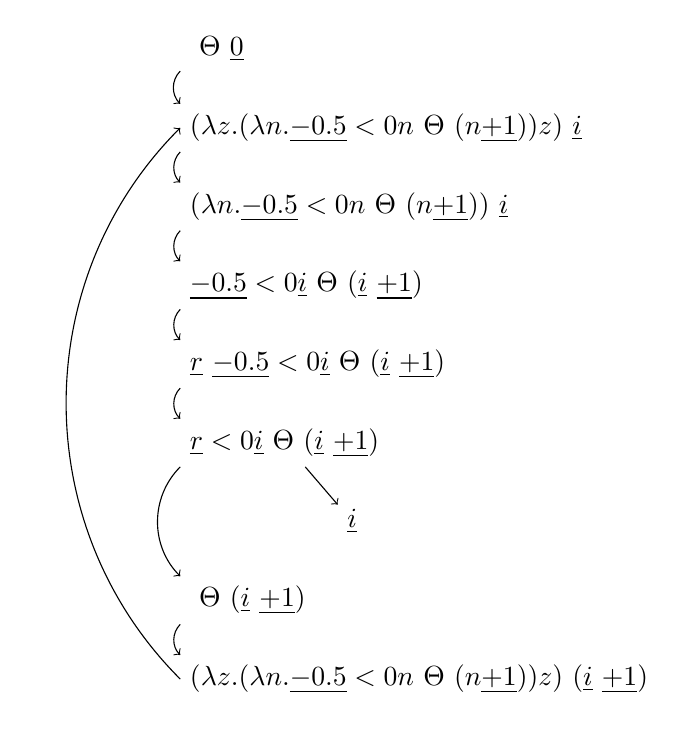
\begin{tikzpicture}[node distance=0.5em, anchor=west]
    \node (1) at (0,-0) {$\tY\ \Theta\ \underline 0$};
    \node (2) at (0,-1) {$(\lambda z. (\lambda n. \tif{\tsample \underline{- 0.5} < 0}{n}{\tY\ \Theta\ (n \underline{+ 1})}) z)\ \underline i$};
    \node (3) at (0,-2) {$(\lambda n. \tif{\tsample \underline{- 0.5} < 0}{n}{\tY\ \Theta\ (n \underline{+ 1})})\ \underline i$};
    \node (4) at (0,-3) {$\tif{\tsample \underline{- 0.5} < 0}{\underline i}{\tY\ \Theta\ (\underline i\ \underline{+ 1})}$};
    \node (5) at (0,-4) {$\tif{\underline r\ \underline{- 0.5} < 0}{\underline i}{\tY\ \Theta\ (\underline i\ \underline{+ 1})}$};
    \node (6) at (0,-5) {$\tif{\underline r < 0}{\underline i}{\tY\ \Theta\ (\underline i\ \underline{+ 1})}$};
    \node (7) at (2,-6) [text width=] {$\underline i$};
    \node (8) at (0,-7) {$\tY\ \Theta\ (\underline i\ \underline{+ 1})$};
    \node (9) at (0,-8) {$(\lambda z. (\lambda n. \tif{\tsample \underline{- 0.5} < 0}{n}{\tY\ \Theta\ (n \underline{+ 1})}) z)\ (\underline i\ \underline{+ 1})$};
    
    \draw [->] (1.south west) to [bend right=45] (2.north west);
    \draw [->] (2.south west) to [bend right=45] (3.north west);
    \draw [->] (3.south west) to [bend right=45] (4.north west);
    \draw [->] (4.south west) to [bend right=45] (5.north west);
    \draw [->] (5.south west) to [bend right=45] (6.north west);
    \draw [->] (6.south west) to [bend right=45] (8.north west);
    \draw [->] (8.south west) to [bend right=45] (9.north west);
    
    \draw [->] (9.west) to [bend left=45] (2.west);
    \draw [->] (6) to (7);
\end{tikzpicture}
\caption{Some reachable terms of $\tY\ \Theta\ \underline 0$\label{fig:geometric distribution}}
\end{figure}
\end{example}

Even in this simple case, defining a ranking function explicitly is awkward because of the number of cases, although in most cases, because the value need only be greater than or equal to that of the next term in sequence, it suffices to take the ranking function as having the same value as the next term, so that overall it takes only 3 distinct values.
(We will explain why later.)

The definition of rankability is also inconvenient for syntactic sugar. It could be useful, for example, to define $M \oplus_p N = \tif{\tsample - p < 0} M N$, where $M \oplus_p N$ reduces to $M$ or $N$, depending on the first value of $s$\lo{Need a name for $s$.}, with probability $p$ resp.~$(1-p)$. Technically though, it reduces first to $\tif{\underline r - p < 0} M N$ for all $r \in I$, so those terms all need values of the ranking function too.

%\paragraph{}
In both of these cases, there are only some values of the ranking function that are semantically important. 
\begin{definition}
Define a \emph{partial ranking function} on a closed term $M$ to be a partial function $f : Rch(M) \rightharpoonup \mathbb R$ such that
\begin{itemize}
    \item $f(N) \geq 0$ for all $N$ where $f$ is defined.
    \item $f$ is defined at $M$.
    \item For any $N$ in the domain of definition of $f$, evaluation of $N$ will eventually \akr{It would be nicer for this to be only almost certain, to make this more neatly in-between rankability and ast, but that doesn't actually work because of terms reachable with 0 probability. Of course, astness doesn't imply rankability, so any definition of partial ranking function that includes all Y-past terms wouldn't always extend to a total ranking function.} reach some $O$ which is either a value or in the domain of definition of $f$, and $f(N) \geq \mathbb E[f(O) + \text{ the number of $\tY$-reduction steps from $N$ to $O$}]$ (where $f(O)$ is taken to be 0 if $O$ is a value outside of the domain of $f$).
\end{itemize}
\end{definition}
A partial ranking function that is total is just a ranking function. Providing a partial ranking function is essentially part way between providing a ranking function and directly proving almost sure termination.

\begin{theorem} \label{thm:partial implies rankable}
Every partial ranking function is a restriction of a ranking function.
\end{theorem}
\begin{proof}
Take a closed term $M$ and partial ranking function $f$ on $M$. Define $f_1 : Rch(M) \rightharpoonup \mathbb R$ by
\begin{align*}
    f_1(N) & := f(N) \text{ whenever $f(N)$ is defined,} \\
    f_1(V) & := 0 \text{ for values $V$ not in the domain of $f$.}
\end{align*}

Define $(\nnext(N,s),\_) = \red^n(N,s)$ for the least $n \geq 0$ such that it's in the domain of $f_1$, and $g(N,s) := \left | \{m < n \mid \red^m(N,s) \text{ is of the form } (E[\tY N'],s') \} \right |$. 
The function $\nnext$ is well-defined (i.e.~$n$ is finite) for all $N \in Rch(M)$ by induction on the path from $M$ to $N$, by the third condition on partial ranking functions. Define $f_2(N) = \int_\entrosp f_1(\nnext(N,s)) + g(N,s) \, \mu_{\entrosp}(\mathrm d s)$. The (total) function $f_2$ agrees with $f$ on $f$'s domain, and it is a ranking function on $M$ (in fact, the least ranking function of which $f$ is a restriction).
\lo{TODO. The preceding sentence deserves a proof.}
\end{proof}


As a corollary, any term which admits a partial ranking function terminates almost surely.

\subsection{Examples}
Let $M \oplus_p N = \tif{\tsample - p < 0} M N$, for $p \in (0,1]$, then there are the pseudo-reduction relations
\begin{align*}
E[M \oplus_p N] \to^3 & E[M] & \\
E[M \oplus_p N] \to^3 & E[N] & \\
\red^3(E[M \oplus_p N], s) = & \left\{
    \begin{array}{ll}
        (E[M],\pi_t(s)) & \text{if } \pi_h(s) < p \\
        (E[N],\pi_t(s)) & \text{if } \pi_h(s) \geq p. \\
    \end{array} \right .
\end{align*}
A partial ranking function could be defined with respect to this shortcut reduction simply by replacing $\to$ and $\red$ in the definition of a partial ranking function by a version that goes straight from $N \oplus_p O$ to $N$ or $O$. Such a pseudo-partial ranking function would then be a partial function from a subset of $Rch(M)$, so it could also be considered as a partial function from all of $Rch(M)$, and it would in fact also be an actual partial ranking function. It is therefore possible to prove rankability directly using the shortcutted reductions.

A similar procedure would work for other forms of syntactic sugar. If a closed term $N$ eventually reduces to one of a set of other terms $\{N_i \mid i \in I\}$ with certain probabilities, a partial ranking function defined with respect to a reduction sequence that skips straight from $N$ to $N_i$ is also a valid partial ranking function for the original reduction function, and therefore its existence implies almost sure termination. There is a caveat, however, that $\tY$-reduction steps skipped over in the shortcut still need to be counted for the expected number of $\tY$-reduction steps.

%\paragraph{}
With this abbreviation, the geometric distribution example from earlier can be written as $(\tY \lambda f n.\ n \oplus_{0.5} f(n+1)) \, \underline 0$. It is then easy to see that the following is a partial ranking function:
\begin{align*}
(\tY \lambda f n.\ n \oplus_{0.5} f(n+1))\ N & \mapsto 2 \\
\underline i \oplus_{0.5} (\tY \lambda f n.\ n \oplus_{0.5} f(n+1))\ (\underline i + 1) & \mapsto 1 \\
\underline i & \mapsto 0.
\end{align*}

In fact, even the partial function $\tY \Theta N \mapsto 2$ alone is a partial ranking function for this term.
